\documentclass{article}

\usepackage{amsmath}
\usepackage{graphicx}
\usepackage{xcolor}
\usepackage[export]{adjustbox}
\RequirePackage[margin=1in]{geometry}

\newcommand\todo[1]{\textcolor{red}{TODO: #1}}

\newcommand\animation[1]{\textcolor{blue}{ANIMATION: #1}}

\begin{document}
	
\title{Hillshade Video Script}
\author{Nathan Stouffer}
\date{}
\maketitle

\section{Intro}

\subsection{Motivation}

What I'm showing you right now is a map.
But you probably didn't need to be told that.
In fact, I would be willing to bet that you not only recognized this as a map, you also instantly discerned many features about this region.
You can probably see that this particular spot is relatively flat and that this other area is pretty steep, that this is a small gully and this is a ridgeline, or maybe that this face is pretty rugged while this slope is not quite as technical.

You are able to get all that complex information from a pretty simple grayscale image -- despite the fact that there is no precise information like contour lines.
In fact, I would be willing to bet that your understanding of this map is better than if I had given you the contour lines even though that is a more precise way to convey information.

\animation{Bring in more maps (one with just contours and another with contours/hillshade)}

Here is a side-by-side to compare.

That is all by design.
The map is intentionally set up so that your brain can intuit all that information.
Modern computers do much of this work today, but cartographers have been using versions of this technique for hundreds of years.
And many other applications use similar strategies to help convey geometric information to your brain.

The thing I'd like to discuss today is called hillshading.
We're going to talk about why it's such an effective method of lighting terrain and walk through the math that powers it.

\begin{center}
	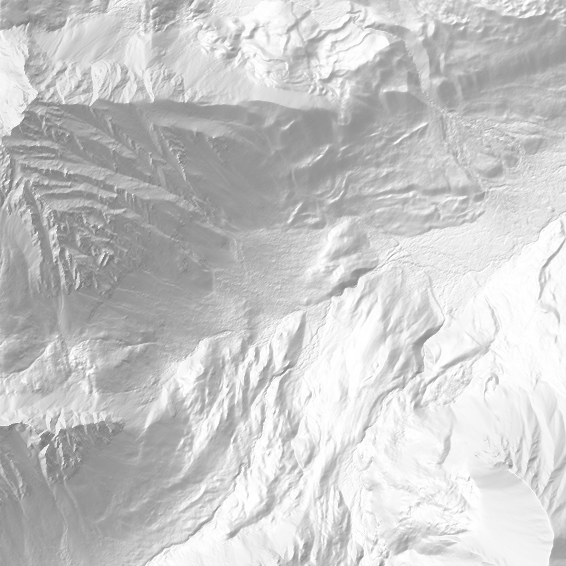
\includegraphics[width=0.5\textwidth,frame]{assets/hillshade-example.png}
\end{center}

\subsection{Directional Lighting}



\subsection{The Puzzle}

\todo{Probably remove this section -- I don't think this section is going to work. By introducing the final product at the beginning of the video, we kind of ruin the mystery of the problem. I am choosing the intro over this puzzle.}

\subsubsection{The Problem}

Say you are some cartographer making maps for adventurers.
Your goal is to produce maps that help people understand a particular area.
Essentially, your goal is to convey information.
You have done research on some area, you know what it looks like.
And you want to record that information in such a way that anyone can read it and understand what is going on.
The medium that you happen to use is a map.
So you want to put all your craft into producing a map that is easy for people to understand.

But, you have a problem.
Many maps
Your map is inherently 2D and the terrain is 3D.

\subsubsection{The spark}

Well, you think, everything people perceive with their eyes is essentially in 2-dimensions anyways.
Your brain is really just receiving signals from your eyes and you reconstruct the 3-dimensional object inside your head.
What convinces us that things are 3D is the difference in colors as the object moves.

That's really all you need to replicate.
And, do you really need to replicate it?
Maybe we can just evoke the essence of that lighting and rely on people's brain to fill in the gaps?

\section{Directional Lighting}

\subsection{Light Direction}

\subsection{Surface Normal}

\subsection{Cosine}

\todo{We can derive $\cos \theta$ by computing the percentage of directional light that hits a small square based on its surface normal.
That follows pretty directly from the definition of $\cos$.}

\todo{This is probably the spot to remap $[-1, 1]$ to $[0, 1]$. It is a small piece of the puzzle but this might be a good spot to introduce it.}

\subsection{Law of Cosines $=>$ Dot Product}

We now know that we want to vary the strength of our lighting according to $\cos \theta$.
But that doesn't really help us much because we don't know what $\theta$ is.
All we know are the vectors $l$ and $n$.
At the end of the day, those are just lists of numbers.
Sure, they have some constraints (like the fact that their length is 1).
And they also have some geometric meaning (they are directions in 3d space).
But when it comes down to it, we need to turn two lists of numbers into something as complex as the cosine function.
How are we supposed to do it?
What is the link between these two vectors and cosine?

If you were some early mathematician, at this point in the proof, you would have to start experimenting with ideas and wait for inspiration to strike.
This sort of thing takes practice and lots of dead ends to feel out.
It's sort of one of those things where experience is the best teacher.

... But if I were to offer one piece of advice, I would say it's often worth constructing a triangle and using some of the many theorems about them to reason your way towards your goal.
Maybe it's the types of problems that I tend to interact with, but I find triangles to be a surprisingly effective tool.
In this case, we are going to draw the third leg of our triangle here and use the Law of Cosines.

We can relate $l$ and $n$ with $\cos \theta$ by using the Law of Cosines.
We already have $\theta$ labeled and we know $|l| = |n| = 1$ because we have constructed them to be unit vectors.
To do this, we need to figure out what the third leg of our triangle is.

\todo{the wording in this paragraph could use some work:}
Vectors add by being placed tip to tail.
This means that the vector $w$, which starts at $l$ and ends at $n$, has the following equality $l = n + w => w = l - n$.

\begin{center}
	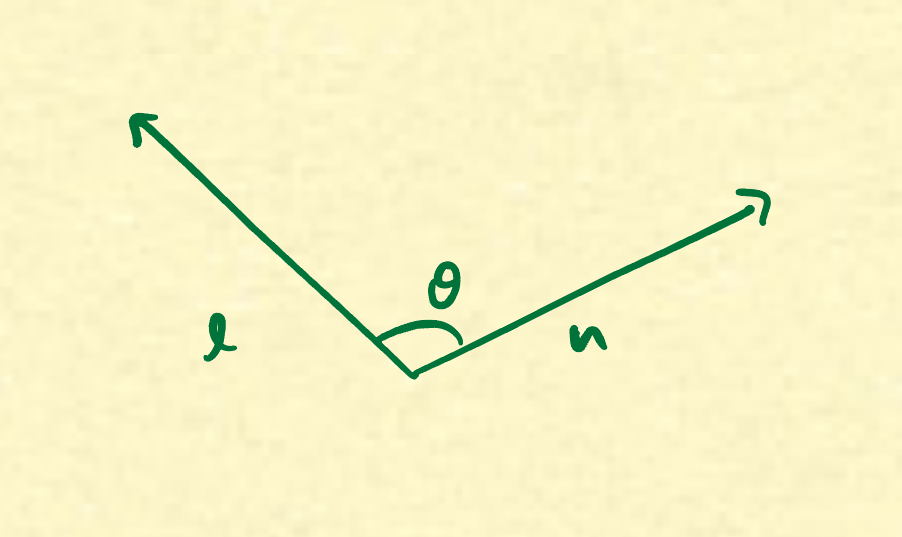
\includegraphics[width=0.3\textwidth,frame]{assets/ln.jpg}
	\hspace{0.2\textwidth}
	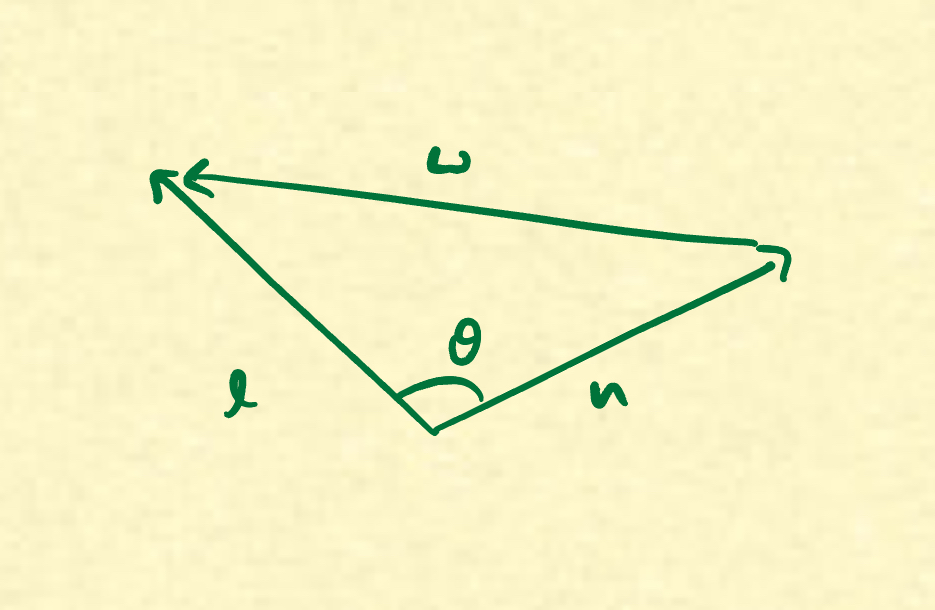
\includegraphics[width=0.2735\textwidth,frame]{assets/lnw.jpg}
\end{center}

The full Law of Cosines says: $c^2 = a^2 + b^2 - 2ab \cos C$.
In our case, $c = | l - n |$, $a = |l|$, $b = |n|$, and $C = \theta$.
So we have:

\begin{align*}
|l-n|^2 = |l|^2 + |n|^2 - 2 |l| |n| \cos \theta & \quad \text{substitute from generalized LoC} \\
|l-n|^2 = 2 - 2 \cos \theta & \quad \text{since we know } |l| = |n| = 1
\end{align*}

\todo{introduce the dot product (but don't call it that)}

\begin{align*}
(l - n) \cdot (l - n) = 2 - 2 \cos \theta & \quad \text{by definition of dot product} \\
l \cdot l - l \cdot n - n \cdot l + n \cdot n = 2 - 2 \cos \theta & \quad \text{by distributive property of dot product} \\
1 - 2 l \cdot n + 1 = 2 - 2 \cos \theta & \quad \text{simplyfying} \\
l \cdot n = \cos \theta & \quad \text{simplifying}
\end{align*}

\subsubsection{Takeaways}

I want you to take away a few things from this proof.

First: The Law of Cosines is true for all triangles -- even degenerate triangles (ones where the three points are co-linear or even identical)!
So no matter what our two vectors are, we can compute the dot product $l \cdot n$ and it will always be $\cos \theta$!

Second: At no point in this proof did we assume the dimension of the vectors involved.
This means that our result holds for any dimension.

Third: We did assume that our two vectors had unit length.
But this relationship also has a more general form.
All we need to do is scale $\cos \theta$ by the lengths of the relevant vectors.
Given any two vectors $ a, b \in \mathbf{R}^n$: $a \cdot b = |a| |b| \cos \theta$.
It might be a fun exercise for you to build on this proof and show why that is the case.

Finally: I'd like you to recognize how surprising and elegant this result is.
I mean, it's crazy that combining two lists of numbers in this really simple way exactly matches $\cos \theta$.
Sometimes simple operations are really powerful.

\section{Hillshade}

So now let's get back to the problem at hand: shading the map.
Given a particular lighting configuration, we know how strongly ...

\section{Endnotes}

\subsection{Modified techniques}

Hillshading isn't just one thing.
It is actually a term for a family of effects that can be applied to a map.
There are a lot of variations out there, and you now have the mathematical framework that sits behind all of them.
Some examples include ambient lighting, exaggerating the normal vector, using multiple light sources, and playing around with colored lights.

\todo{Possibly mention Eduard Imhof.}

\subsection{Pseudoscopic Illusion}

In mapping, the light source for hillshade is typically placed in the northwest.
This is because many maps use a north-up convention, placing the light source in the top left.
Broadly speaking, people recognize features better when this is the case.

However, this can some backfire when a map with static hillshade is oriented with a south-up convention.
When that occurs, your brain might interpret everything backwards (valleys as ridges and ridges and valleys).
This is called a pseudoscopic illusion.

\animation{Show a south-up map light from the northwest and then fade in the same map (still south up) with a southeast (top left) light}.

\subsection{2D vs 3D}

I'd like to end the video by making one last comment on the simplicity of this effect: this is not a 3-dimensional map.
And I don't just mean that the screen you're viewing is 2-dimensional.
I mean that the actual model that I am rendering is 2D.

\animation{Pitch the camera}

Despite that, it is an incredibly effective method of conveying terrain information.
I find that fascinating.

\animation{3D flythrough?}

\end{document}